A data set of 57 consecutive measurements from a machine tool are in the TSA package.
\begin{enumerate}[label=(\alph*)]
    \item Estimate the parameters of a (mean-centered) AR(1) model for this series. Use the least
squares method and maximum likelihood, and report the estimated parameters from each of
these methods. Comment on any similarities and differences. Give the confidence intervals of
your parameters.
    \item Estimate the parameters of a (mean-centered) AR(2) model for this series. Use the least
squares method and maximum likelihood, and report the estimated parameters from each of
these methods. Comment on any similarities and differences.
    \item Derive the confidence intervals for the parameters $\phi_1$ and $\phi_2$. Does the confidence interval for $\phi_2$ suggests it should be included in the model?
    \item Compare the results of the maximum likelihood fits from parts (a) and (b). Which model
do you believe is preferable? Briefly explain your answer.
    \item Perform a diagnostic check of the residuals. Comments.
    \item Compare the two models using AIC, BIC. Which one do you prefer? Does any of the
quantities suggests one model is better than the other? If so, how much do you gain in errors reduction if any. Is that in line with your answer in (d)?
\end{enumerate}

\subsection{R Code}
\lstinputlisting[language=R]{Codes/Midterm_2_P2.R}
\newpage
\subsection{Results}
\begin{figure}[!htb]
    \centering
    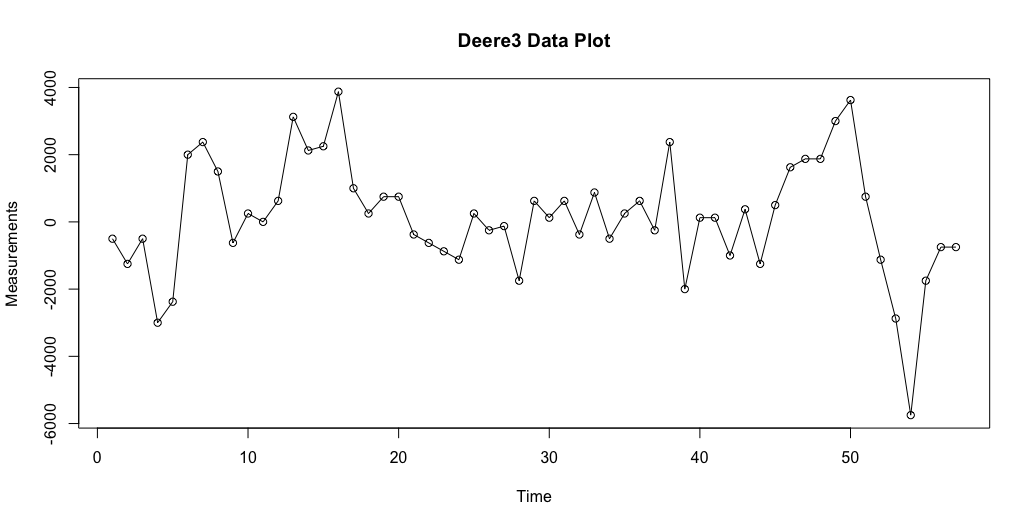
\includegraphics[width=0.9\linewidth]{Images/P2/TS_Plot_P2.png}
    \caption{Time series plot of the Deere3 data.}
    \label{fig:deere3}
\end{figure}
\begin{enumerate}[label=(\alph*)]
    \item Least squares method for AR(1) parameter estimation: \small\begin{block}
> print(css_model_ar1_coef)
        ar1   intercept 
  0.5332044 160.0797248 
> confint(css_model_ar1)
                 2.5 %      97.5 %
ar1          0.3132122   0.7531966
intercept -646.0111173 966.1705670
\end{block}
\normalsize Maximum Likelihood method for AR(1) parameter estimation: \small\begin{block}
> print(ml_model_ar1_coef)
        ar1   intercept 
  0.5255778 124.3524257 
> confint(ml_model_ar1)
                 2.5 %      97.5 %
ar1          0.3084104   0.7427452
intercept -648.3281895 897.0330409
\end{block}
\normalsize The estimated $\hat\phi$ from both the least squares and maximum likelihood methods are very similar. However, the intercept ($\hat\mu$) is significantly different. In addition, the confidence intervals for $\hat\phi$ in both cases are similar and $0 \not\in$ CI($\hat\phi$). 
    \item Least squares method for AR(2) parameter estimation: \small\begin{block}
> print(css_model_ar2_coef)
         ar1          ar2    intercept 
5.245848e-01 7.938728e-03 2.011876e+02 
\end{block}
\normalsize Maximum Likelihood method for AR(2) parameter estimation: \small\begin{block}
> print(ml_model_ar2_coef)
         ar1          ar2    intercept 
  0.52111096   0.00830321 123.24182209 
\end{block}
\normalsize Like before, the estimated $\phi_1$ and $\phi_2$ in both cases are pretty similar, whereas, the intercepts are significantly different. 
\item Confidence intervals for $\phi_1$ and $\phi_2$: \small\begin{block}
Least Squares Method
> confint(css_model_ar2)
                 2.5 %       97.5 %
ar1          0.2660503    0.7831192
ar2         -0.2509164    0.2667939
intercept -607.0745845 1009.4498459

Maximum Likelihood Method
> confint(ml_model_ar2)
                 2.5 %      97.5 %
ar1          0.2642641   0.7779579
ar2         -0.2493401   0.2659465
intercept -656.0388502 902.5224944
\end{block}
\normalsize Since $0 \in$ CI($\phi_2$), therefore, $\phi_2 \approx 0$. So $\phi_2$ should not be included in the model.
\item \label{answer_ref_d} The maximum likelihood estimates of the intercepts for the AR(1) and AR(2) models are pretty similar. Also, the confidence interval of the intercept in case of AR(1) is a subset of that of AR(2). But, since our target is develop a parsimonious model and $0 \in$ CI($\phi_2$) for the maximum likelihood method as well, so, AR(1) is the preferable model. 

\item Residual Diagnostics:
\begin{figure}[!htb]
    \centering
    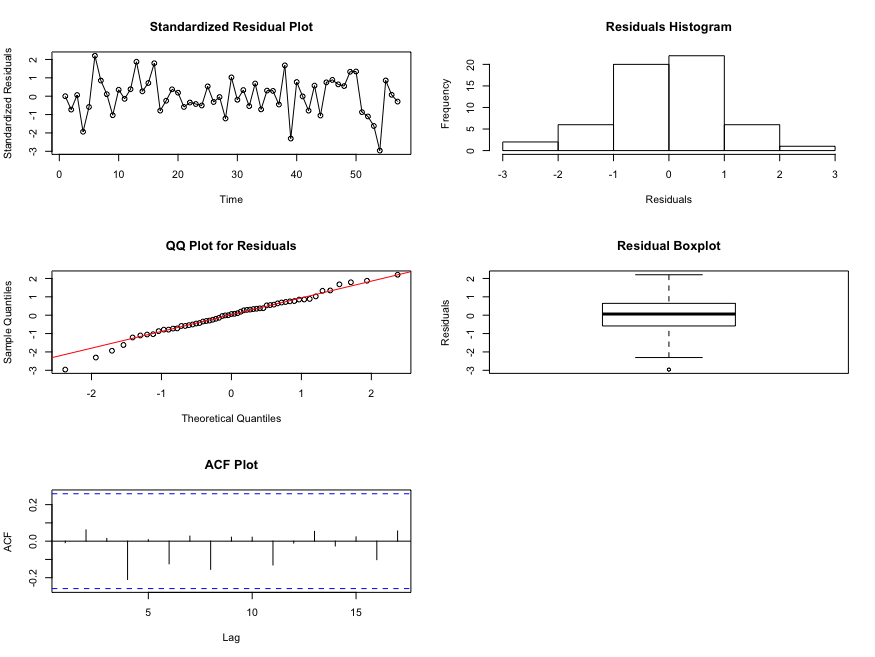
\includegraphics[width=\linewidth]{Images/P2/Residual_CSS_AR1.png}
    \caption[Residual diagnostic plots for least squares estimation for AR(1).]{Residual diagnostic plots for least squares estimation for AR(1). These plots shows that the residuals tend to closely follow a normal distribution.}
    \label{fig:residual_css_ar1}
\end{figure}
\begin{figure}[!htb]
    \centering
    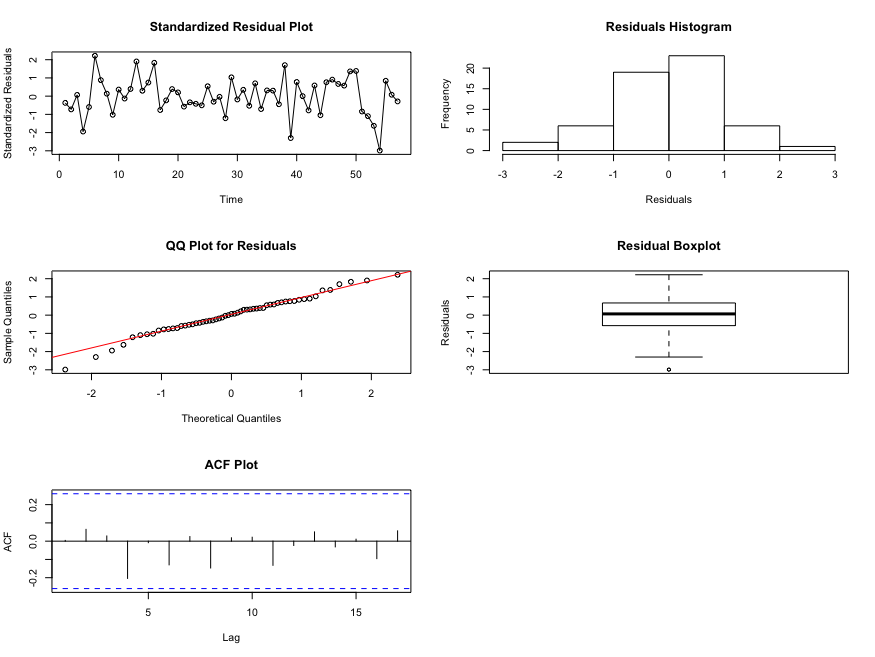
\includegraphics[width=\linewidth]{Images/P2/Residual_ML_AR1.png}
    \caption[Residual diagnostic plots for maximum likelihood estimation for AR(1)]{Residual diagnostic plots for maximum likelihood estimation for AR(1). Similar observations like that of Fig \ref{fig:residual_css_ar1} can be made.}
\end{figure}
\begin{figure}[!htb]
    \centering
    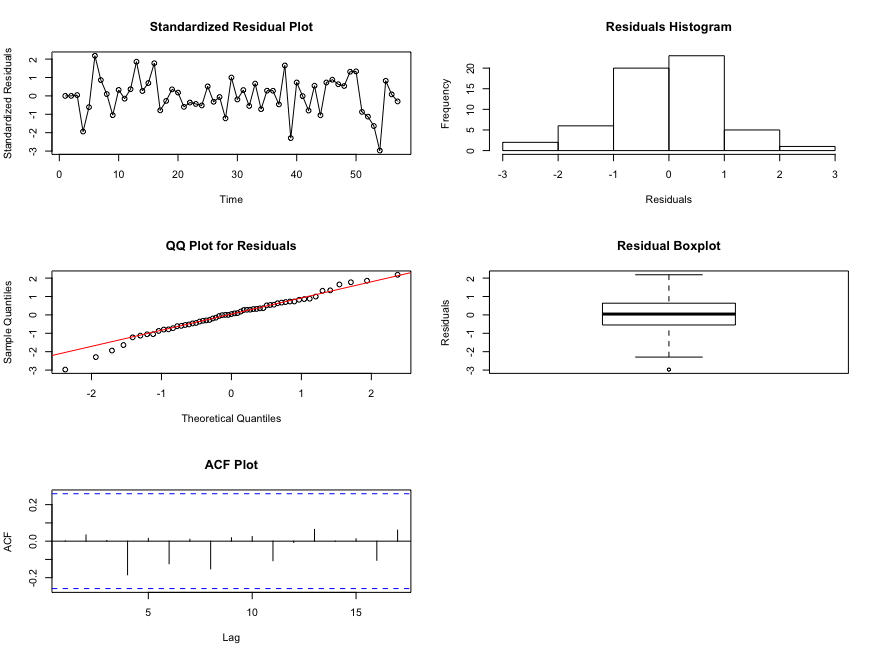
\includegraphics[width=\linewidth]{Images/P2/Residual_CSS_AR2.png}
    \caption[Residual diagnostic plots for least squares estimation for AR(2).]{Residual diagnostic plots for least squares estimation for AR(2). Like before, these also closely follow a normal distribution but less than AR(1) residuals.}
    \label{fig:residual_css_ar2}
\end{figure}
\begin{figure}[!htb]
    \centering
    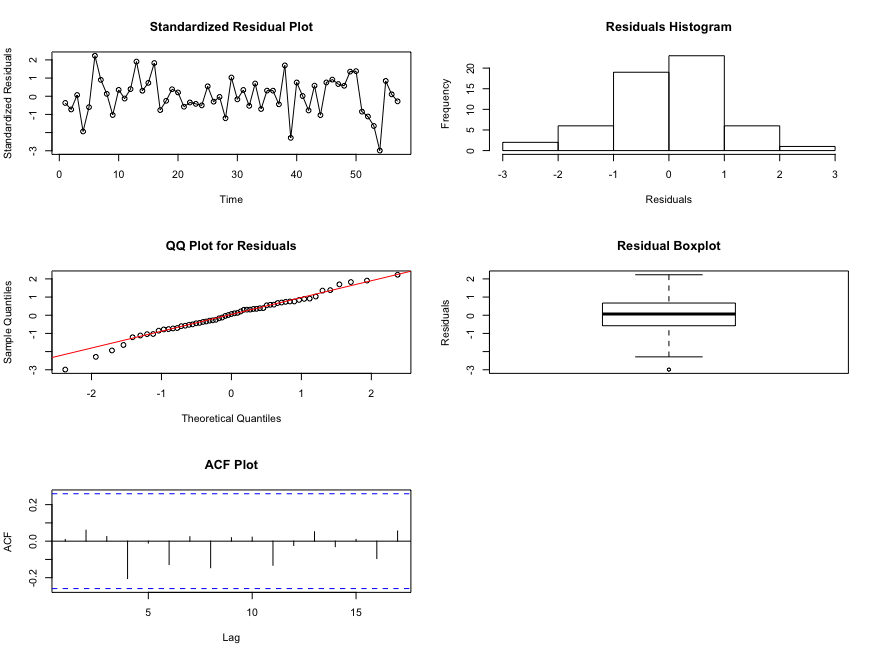
\includegraphics[width=\linewidth]{Images/P2/Residual_ML_AR2.png}
    \caption[Residual diagnostic plots for maximum likelihood estimation for AR(2).]{Residual diagnostic plots for maximum likelihood estimation for AR(2). Similar observations like that of Fig \ref{fig:residual_css_ar2} can be made.}
\end{figure}
The residual normality test results are given below. \small\begin{block}
Least Squares Estimation for AR(1):

Shapiro-Wilk normality test
data:  st_residuals
W = 0.98297, p-value = 0.6

Exact runs test
data:  st_residuals
Runs = 29, p-value = 1

Maximum Likelihood Estimation for AR(1):

Shapiro-Wilk normality test
data:  st_residuals
W = 0.98261, p-value = 0.5827

Exact runs test
data:  st_residuals
Runs = 29, p-value = 1

Least Squares Estimation for AR(2):

Shapiro-Wilk normality test
data:  st_residuals
W = 0.9809, p-value = 0.5028

Exact runs test
data:  st_residuals
Runs = 29, p-value = 1

Maximum Likelihood Estimation for AR(2):

Shapiro-Wilk normality test
data:  st_residuals
W = 0.98294, p-value = 0.599

Exact runs test
data:  st_residuals
Runs = 29, p-value = 1
\end{block}
\normalsize The normality tests show that the residuals from the AR(1) tend to follow the normal distribution more closely than those of AR(2).
\item AIC and BIC tests for the maximum likelihood method: \small\begin{block}
AR(1):
> AIC(model)
[1] 997.0189
> BIC(model)
[1] 1003.148

AR(2):
> AIC(model)
[1] 999.0148
> BIC(model)
[1] 1007.187
\end{block}
\normalsize As observed, we obtain a reduction of $\approx 2$ and $\approx 4$ in the AIC and BIC values respectively for the AR(1) model. Although, these are not significant reductions, our aim is always to develop a parsimonious model which aligns with the results obtained in \ref{answer_ref_d}. Therefore, AR(1) is the preferred model which is further confirmed using the auto.arima function in R.
\small\begin{block}
> auto_arima
Series: deere3 
ARIMA(1,0,0) with zero mean 

Coefficients:
         ar1
      0.5291
s.e.  0.1103

sigma^2 estimated as 2109761:  log likelihood=-495.56
AIC=995.12   AICc=995.34   BIC=999.2
\end{block}
\end{enumerate}